\section{Numerical Methods -- Multiple Variable Quasi-Newton Method}
This chapter formally presents the Newton-Raphson method as the preferred alternative to using an optimizer routine to solve systems of non-linear equations.
The method is used later in the document to solve for flows and heads in a pipeline network.

Lets return to our previous example where the function \textbf{f} is a vector-valued function of a vector argument.

\begin{gather}
\mathbf{f(x)} = 
\begin{matrix}
f_1 = & x^2 & +~y^2 & - 4\\
f_2 = & e^x & +~y  & - 1\\
\end{matrix}
\end{gather}

Lets also recall Newtons method for scalar valued function of a single variable.

\begin{equation}
x_{k+1}=x_{k} - \frac{  f(x_{k})  }{   \frac{df}{dx}\rvert_{x_k} } 
\label{eqn:NewtonFormula}
\end{equation}

Extending to higher dimensions, the value $x$ become the vector \textbf{x} and the function $f()$ becomes the vector function \textbf{f()}.
What remains is an analog for the first derivative in the denominator (and the concept of division of a matrix).

The analog to the first derivative is a matrix called the Jacobian which is comprised of the first derivatives of the function \textbf{f} with respect to the arguments \textbf{x}.   
For example for a 2-value function of 2 arguments (as our example above)

\begin{equation}
\frac{df}{dx}\rvert_{x_k} =>
\begin{pmatrix}
\frac{\partial f_1}{\partial x_1} & \frac{\partial f_1}{\partial x_2} \\
~ & ~ \\
\frac{\partial f_2}{\partial x_1} & \frac{\partial f_2}{\partial x_2} \\
\end{pmatrix}
\label{eqn:Jacobian}
\end{equation}

Next recall that division is replaced by matrix multiplication with the multiplicative inverse, so the analogy continues as

\begin{equation}
\frac{1}{\frac{df}{dx}\rvert_{x_k}} =>
{\begin{pmatrix}
\frac{\partial f_1}{\partial x_1} & \frac{\partial f_1}{\partial x_2} \\
~ & ~ \\
\frac{\partial f_2}{\partial x_1} & \frac{\partial f_2}{\partial x_2} \\
\end{pmatrix}}^{-1}
\label{eqn:JacobianInverse}
\end{equation}

Lets name the Jacobian \textbf{J(x)}.

So the multi-variate Newton's method can be written as

\begin{equation}
\mathbf{x}_{k+1}=\mathbf{x}_{k} - \mathbf{J(x)}^{-1}\rvert_{x_k} \cdot \mathbf{f(x)}\rvert_{x_k}
\label{eqn:VectorNewtonFormula}
\end{equation}

In the linear systems chapter we did find a way to solve for an inverse, but its not necessary -- a series of rearrangement of the system above yields a nice scheme tthat does not require inversion of a matrix.

First, move the $\mathbf{x}_{k}$ to the left-hand side.

\begin{equation}
\mathbf{x}_{k+1}-\mathbf{x}_{k} = - \mathbf{J(x)}^{-1}\rvert_{x_k} \cdot \mathbf{f(x)}\rvert_{x_k}
\label{eqn:VectorNewtonFormula}
\end{equation}

Next multiply both sides by the Jacobian. 

\begin{equation}
\mathbf{J(x)}\rvert_{x_k} \cdot (\mathbf{x}_{k+1}-\mathbf{x}_{k}) = - \mathbf{J(x)}\rvert_{x_k} \cdot \mathbf{J(x)}^{-1}\rvert_{x_k} \cdot \mathbf{f(x)}\rvert_{x_k}
\label{eqn:VectorNewtonFormula}
\end{equation}

Recall a matrix multiplied by its inverse returns the identity matrix (the matrix equivalent of unity)

\begin{equation}
- \mathbf{J(x)}\rvert_{x_k} \cdot (\mathbf{x}_{k+1}-\mathbf{x}_{k}) = \mathbf{f(x)}\rvert_{x_k}
\label{eqn:NewtonRaphsonFormula}
\end{equation}

So we now have an algorithm:
\begin{enumerate}
\item Start with an initial guess $\mathbf{x}_{k}$, compute $\mathbf{f(x)}\rvert_{x_k}$, and $\mathbf{J(x)}\rvert_{x_k}$.
\item Test for stopping.  Is $\mathbf{f(x)}\rvert_{x_k}$ close to zero?  If yes, exit and report results, otherwise continue.
\item Solve the linear system $\mathbf{J(x)}\rvert_{x_k} \cdot (\mathbf{x}_{k+1}-\mathbf{x}_{k}) = \mathbf{f(x)}\rvert_{x_k}$.
\item Test for stopping.  Is $ (\mathbf{x}_{k+1}-\mathbf{x}_{k})$ close to zero?  If yes, exit and report results, otherwise continue.
\item Compute the update $\mathbf{x}_{k+1} = \mathbf{x}_{k} - (\mathbf{x}_{k+1}-\mathbf{x}_{k}) $, then
\item Move the update into the guess vector $\mathbf{x}_{k} <=\mathbf{x}_{k+1}$ =and repeat step 1.   Stop after too many steps.
\end{enumerate}

Now to repeat the example from the previous chapter, except we will employ this algorithm.

The function (repeated)

\begin{gather}
\mathbf{f(x)} = 
\begin{matrix}
f_1 = & x^2 & +~y^2 & - 4\\
f_2 = & e^x & +~y  & - 1\\
\end{matrix}
\end{gather}

Then the Jacobian, here we will compute it analytically because we can

\begin{equation}
\mathbf{J(x)}=>
{\begin{pmatrix}
2x & 2y \\
~ & ~ \\
e^x & 1 \\
\end{pmatrix}}
\label{eqn:JacobianExample}
\end{equation}

Listing \ref{lst:NewtonRaphsonMethod} is a listing that implements the Newton-Raphson method with analytical derivatives.

\begin{lstlisting}[caption=R code demonstrating Newton's Method calculations, label=lst:NewtonRaphsonMethod]
# R script for system of non-linear equations using Newton-Raphson with analytical derivatives
# forward define the functions
####### f(x) #########################
func <- function(x_vector){
  func <- numeric(0)
  func[1] <- x_vector[1]^2 + x_vector[2]^2 - 4
  func[2] <- exp(x_vector[1]) + x_vector[2] - 1
  return(func)
}
######## J(x) #########################
jacob <- function(x_vector){
  jacob <- matrix(0,nrow=2,ncol=2)
  jacob[1,1] <- 2*x_vector[1]   ; jacob[1,2] <- 2*x_vector[2];
  jacob[2,1] <- exp(x_vector[1]); jacob[2,2] <- 1 ;
  return(jacob)
}
####### Solver Parameters #############
x_guess <- c(2.,-0.8)
tolerancef <- 1e-9  # stop if function gets to zero
tolerancex <- 1e-9  # stop if solution not changing
maxiter <- 20 # stop if too many iterations
x_now <- x_guess
###### Newton-Raphson Algorithm ########
for (iter in 1:maxiter){
  funcNow <- func(x_now)
  testf <- t(funcNow) %*% funcNow
  if(testf < tolerancef){
    message("f(x) is close to zero : ", testf);
    break
  }
  dx <- solve(jacob(x_now),funcNow)
  testx <- t(dx) %*% dx
  if(testx < tolerancex){
    message("solution change small : ", testx);
    break
  }
  x_now <- x_now - dx
}
#########################################
if( iter == maxiter) {message("Maximum iterations -- check if solution is converging : ")}
message("Initial Guess"); print(x_guess);
message("Initial Function Value: "); print(func(x_guess));
message("Exit Function Value : ");print(func(x_now));
message("Exit Vector : "); print(x_now)
\end{lstlisting}

Figure \ref{fig:NewtonRaphsonAnalytical} implements the script in Listing \ref{lst:NewtonRaphsonMethod} for the example problem.  

The next variant is to approximate the derivatives -- usually a Finite-Difference approximation is used, either forward, backward, or centered differences -- generally determined based on the actual behavior of the functions themselves or by trial and error. 
For really huge systems, we usually make the program itself make the adaptions as it proceeds.

The coding for a finite-difference representation of a Jacobian is shown in Listing \ref{lst:NewtonRaphsonQuasi}.  
In constructing the Jacobian, we observe that each column of the Jacobian is simply the directional derivative of the function with respect to the variable associated with the column.  
For instance, the first column of the Jacobian in the example is first derivative of the first function (all rows) with respect to the first variable, in this case $x$.  The second column is the first derivative of the second function with respect to the second variable, $y$.  
This structure is useful to generalize the Jacobian construction method because we can write (yet another) prototype function that can take the directional derivatives for us, and just insert the returns as columns.
The example listing is specific to the 2X2 function in the example, but the extension to more general cases is evident.

\begin{lstlisting}[caption=R code demonstrating Newton's Method calculations using finite-difference approximations to the partial derivatives, label=lst:NewtonRaphsonQuasi]
# R script for system of non-linear equations using Newton-Raphson with 
#    finite-difference approximated derivatives
#    forward define the functions
####### f(x) #########################
func <- function(x_vector){
  func <- numeric(0)
  func[1] <- x_vector[1]^2 + x_vector[2]^2 - 4
  func[2] <- exp(x_vector[1]) + x_vector[2] - 1
  return(func)
}
######## J(x) #########################
jacob <- function(x_vector,func){  #supply a vector and the function name
# the columns of the jacobian are just directional derivatives 
  dv <- 1e-06 #perturbation value for finite difference
  df1 <- numeric(0);
  df2 <- numeric(0);
  dxv <- x_vector;
  dyv <- x_vector;
# perturb the vectors
  dxv[1] <- dxv[1]+dv;
  dyv[2] <- dyv[2]+dv;
  df1 <- (func(dxv) - func(x_vector))/dv;
  df2 <- (func(dyv) - func(x_vector))/dv;
  jacob <- matrix(0,nrow=2,ncol=2)
# for a more general case should put this into a loop
  jacob[1,1] <- df1[1]   ;  jacob[1,2] <- df2[1]  ;
  jacob[2,1] <- df1[2]   ;  jacob[2,2] <- df2[2]  ;
  return(jacob)
}
####### Solver Parameters #############
x_guess <- c(2.,-0.8)
tolerancef <- 1e-9  # stop if function gets to zero
tolerancex <- 1e-9  # stop if solution not changing
maxiter <- 20 # stop if too many iterations
x_now <- x_guess
###### Newton-Raphson Algorithm ########
for (iter in 1:maxiter){
  funcNow <- func(x_now)
  testf <- t(funcNow) %*% funcNow
  if(testf < tolerancef){
    message("f(x) is close to zero : ", testf);
    break
  }
  dx <- solve(jacob(x_now,func),funcNow)
  testx <- t(dx) %*% dx
  if(testx < tolerancex){
    message("solution change small : ", testx);
    break
  }
  x_now <- x_now - dx
}
#########################################
if( iter == maxiter) {message("Maximum iterations -- check if solution is converging : ")}
message("Initial Guess"); print(x_guess);
message("Initial Function Value: "); print(func(x_guess));
message("Exit Function Value : ");print(func(x_now));
message("Exit Vector : "); print(x_now)
\end{lstlisting}


\begin{figure}[h!] %  figure placement: here, top, bottom, or page
   \centering
   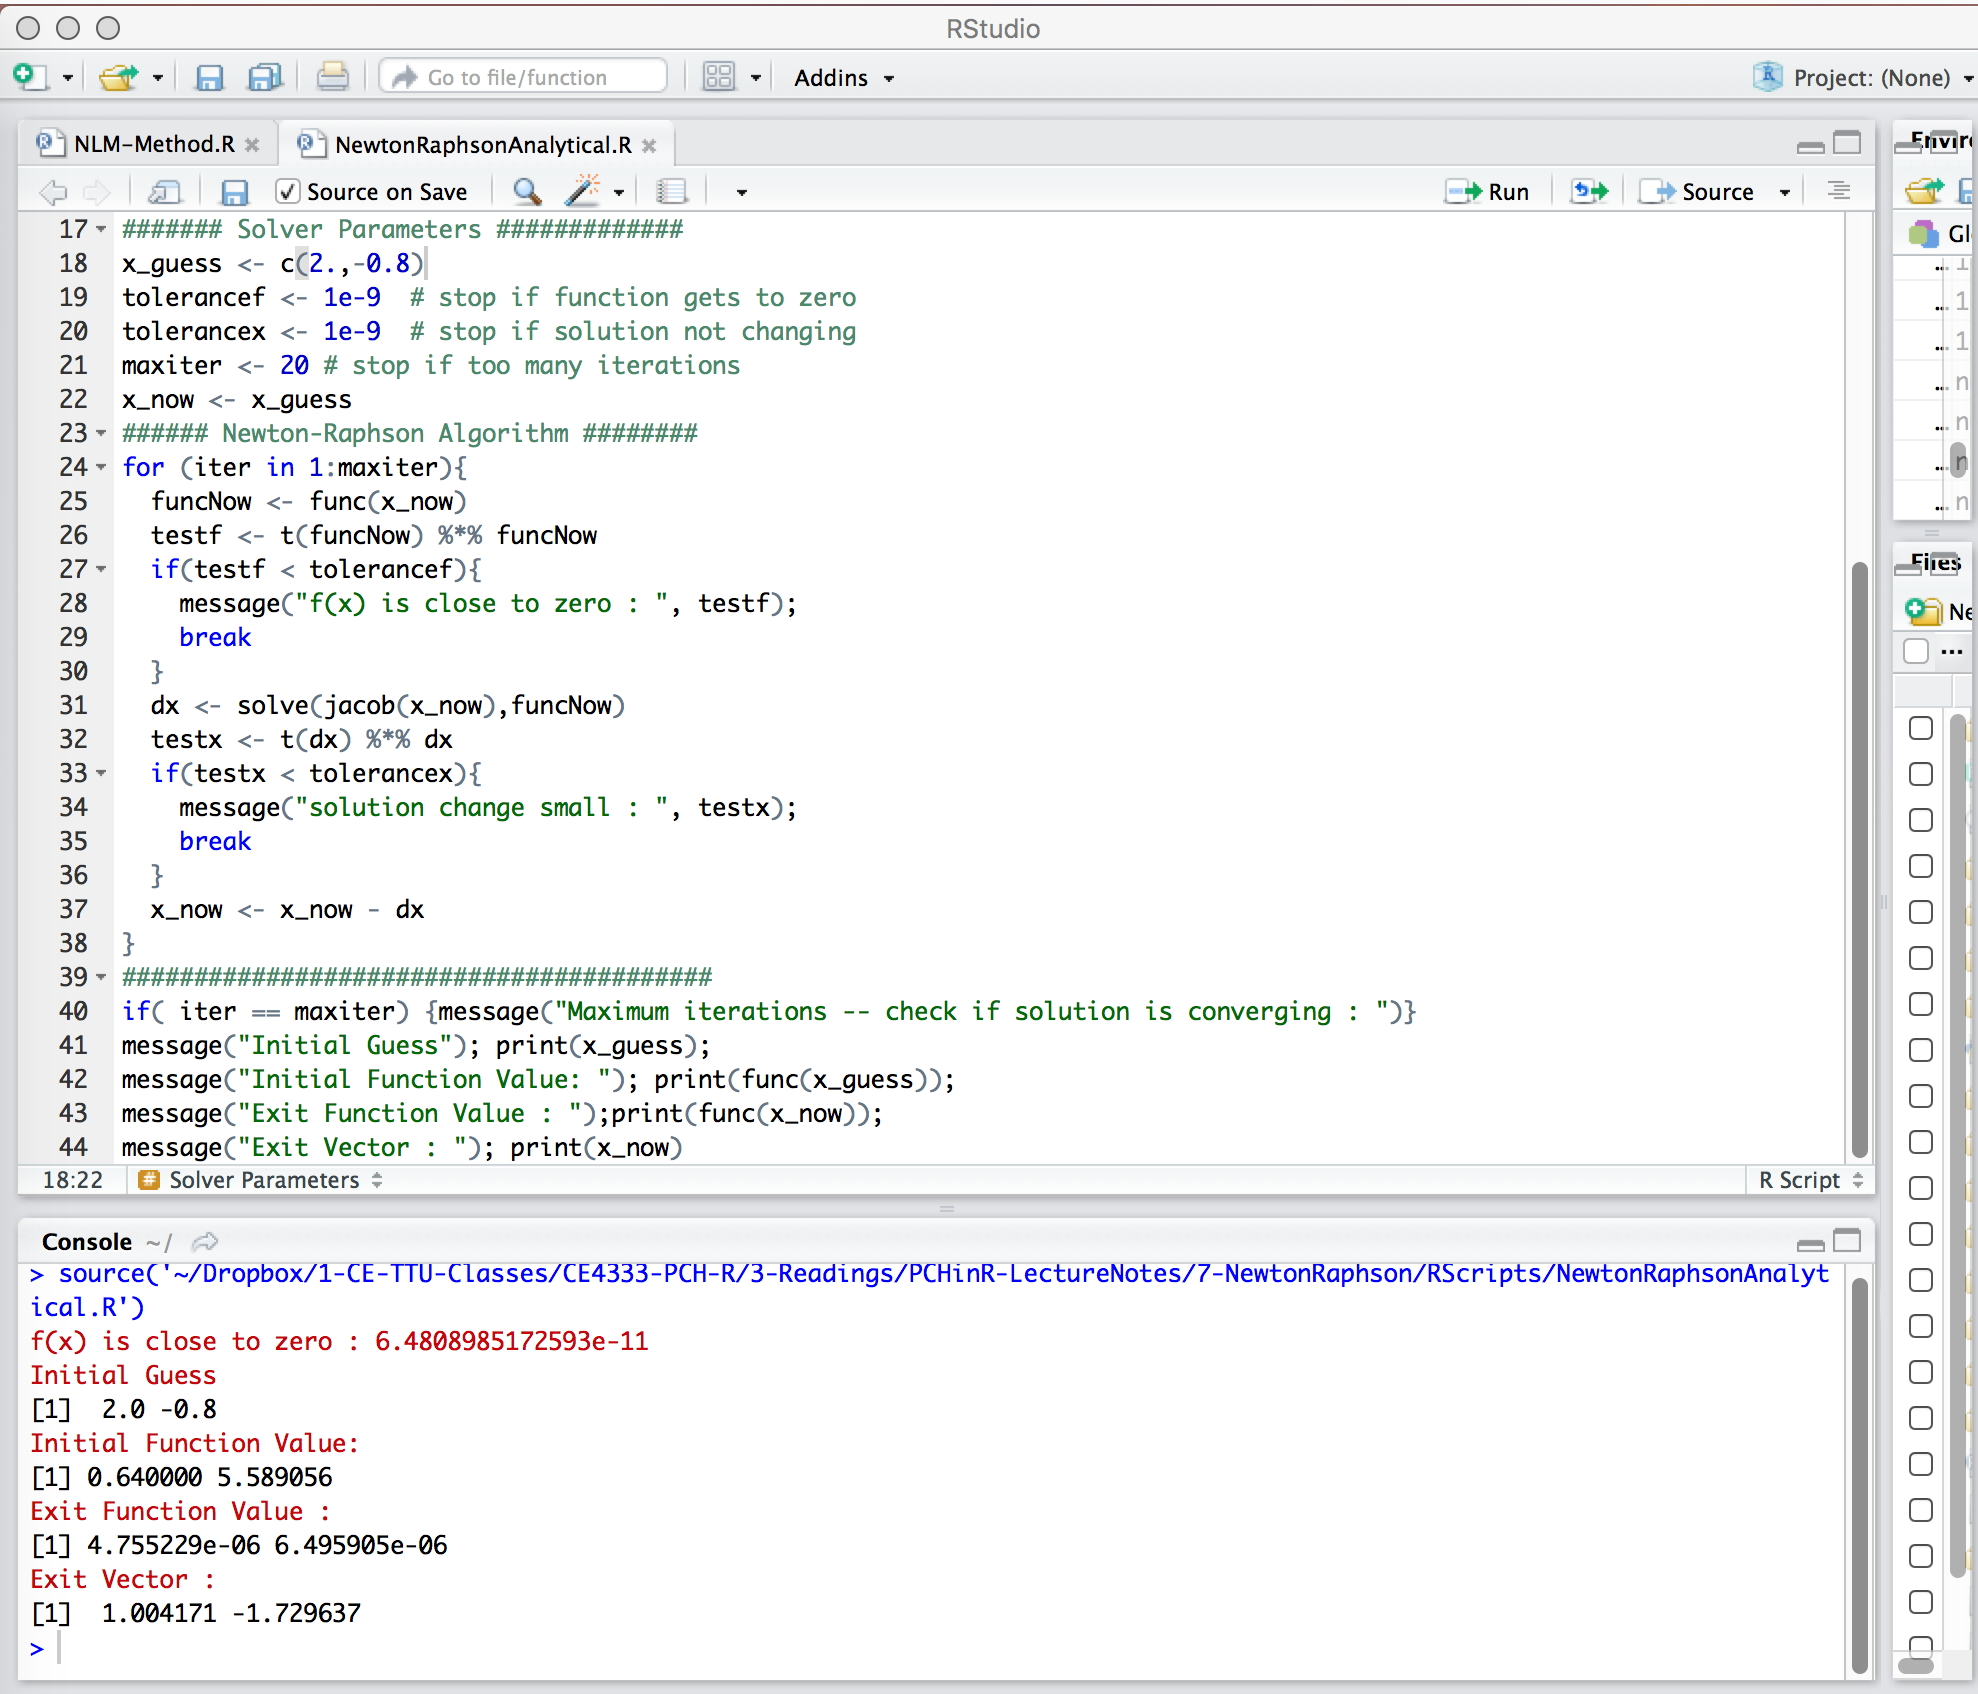
\includegraphics[height=4in]{./7-NewtonRaphson/NewtonRaphsonAnalytical.jpg} 
   \caption{Newton-Raphson using Analytical Derivatives}
   \label{fig:NewtonRaphsonAnalytical}
\end{figure}

\begin{figure}[h!] %  figure placement: here, top, bottom, or page
   \centering
   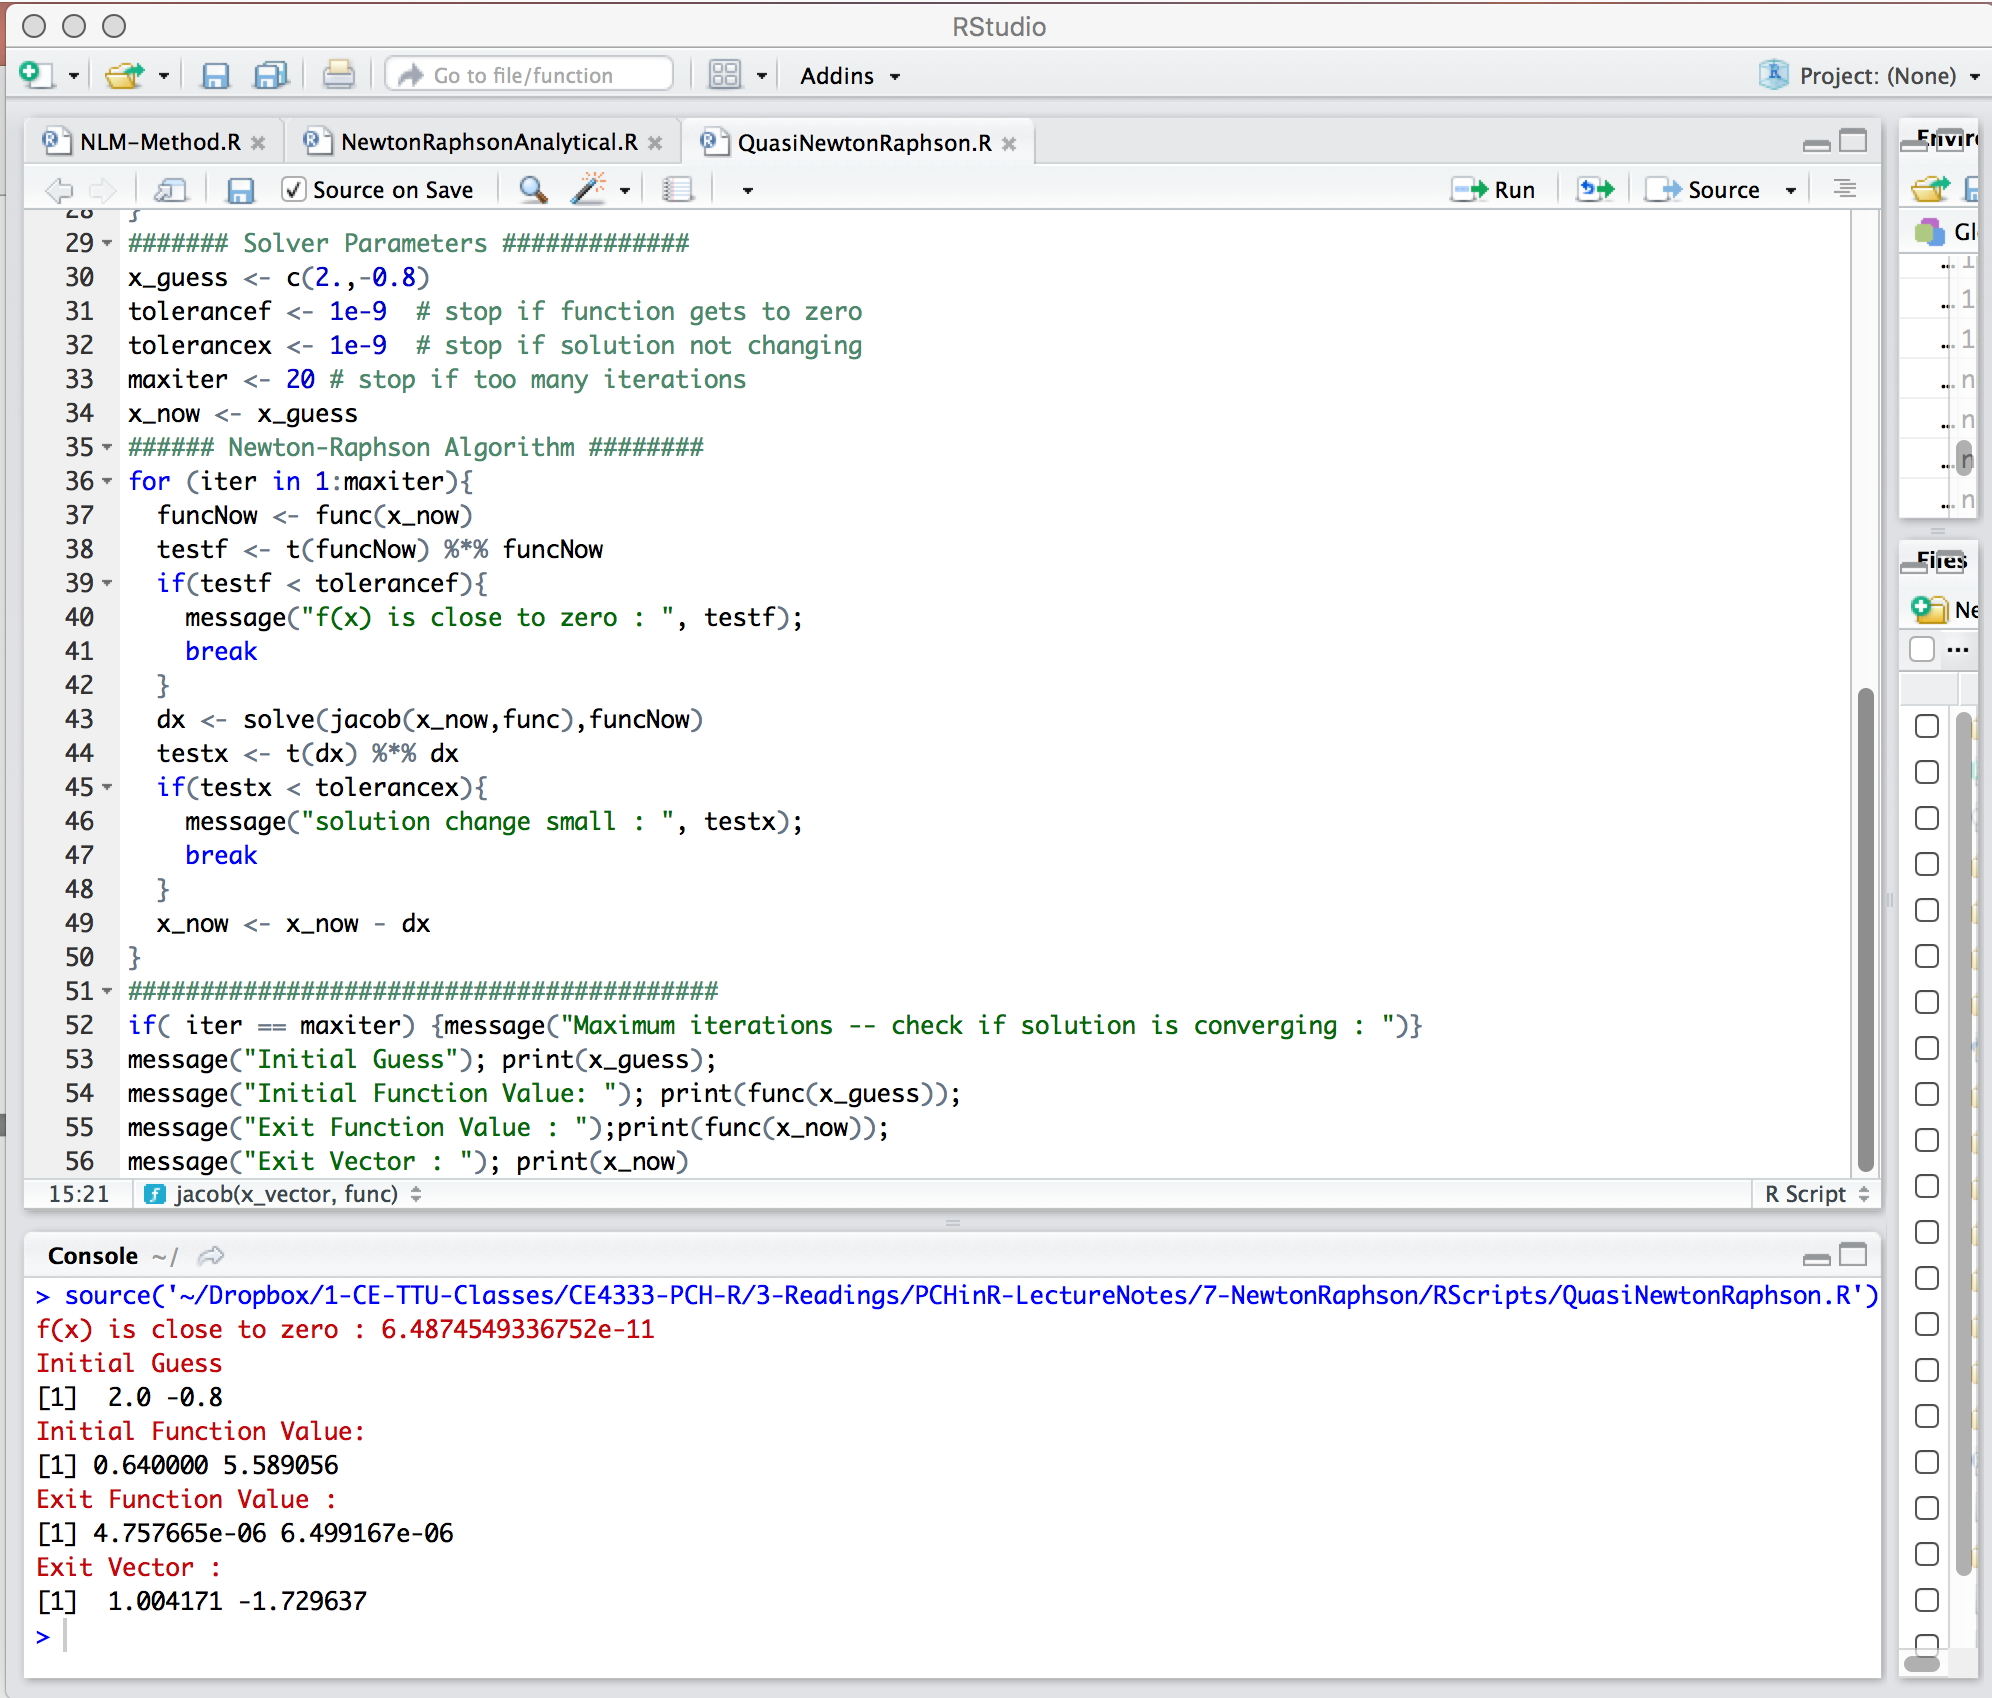
\includegraphics[height=4in]{./7-NewtonRaphson/NewtonRaphsonFiniteDiff.jpg} 
   \caption{Newton-Raphson using Finite-Difference Approximated Derivatives}
   \label{fig:NewtonRaphsonFiniteDiff}
\end{figure}

%\subsection{Exercises}
%\begin{enumerate}
%\item Write a script that forward defines the multi-variate functions and implements the Newton-Raphson technique in \textbf{R}.
%Implement the method, using analytical derivatives, and find a solution to:
%\begin{gather}
%\begin{matrix}
% x^3 & +~3y^2 & = 21\\
%x^2& +~2y  & = -2 \\
%\end{matrix}
%\end{gather}
%\item Repeat the exercise, except use finite-differences to approximate the derivatives.
%\newpage
%\item Write a script that forward defines the multi-variate functions and implements the non-linear minimization technique in \textbf{R}.
%Implement the method, using analytical derivatives, and find a solution to:
%\begin{gather}
%\begin{matrix}
%x^2 & +~ y^2 & +~z^2 & =~ 9\\
%~ & ~ & xyz & =~ 1\\
%x & +~ y & -z^2 & =~ 0\\
%\end{matrix}
%\end{gather}
%\item Repeat the exercise, except use finite-differences to approximate the derivatives.
%\item Write a script that forward defines the multi-variate functions and implements the non-linear minimization technique in \textbf{R}.
%Implement the method, using analytical derivatives, and find a solution to:
%\begin{gather}
%\begin{matrix}
%xyz & -~ x^2 & +~y^2 & =~ 1.34\\
%~ & xy &-~z^2 & =~ 0.09\\
%e^x & -~ e^y & +z & =~ 0.41\\
%\end{matrix}
%\end{gather}
%\item Repeat the exercise, except use finite-differences to approximate the derivatives.
%\end{enumerate}

